\documentclass[11pt]{article}
\usepackage[margin=1in]{geometry}
\usepackage{amsmath, amssymb}
\usepackage{xcolor}
\usepackage{tikz}
\usepackage{pgfplots}
\pgfplotsset{compat=1.16} % Use 1.15 if your TeXLive is older
\usetikzlibrary{arrows.meta,calc}

\begin{document}

\section*{Geometric Sketches (Larger, Clear Callouts Away from Curves)}
Each figure shows the dashed \textcolor{orange!85!black}{secant} approaching the \textcolor{red!75!black}{tangent} as $h\to 0$. Labels are placed in white boxes away from curves, with arrows pointing to the relevant points/lines.

% ===================== Figure 1: f(x)=x^2 =====================
\begin{figure}[p]
\centering
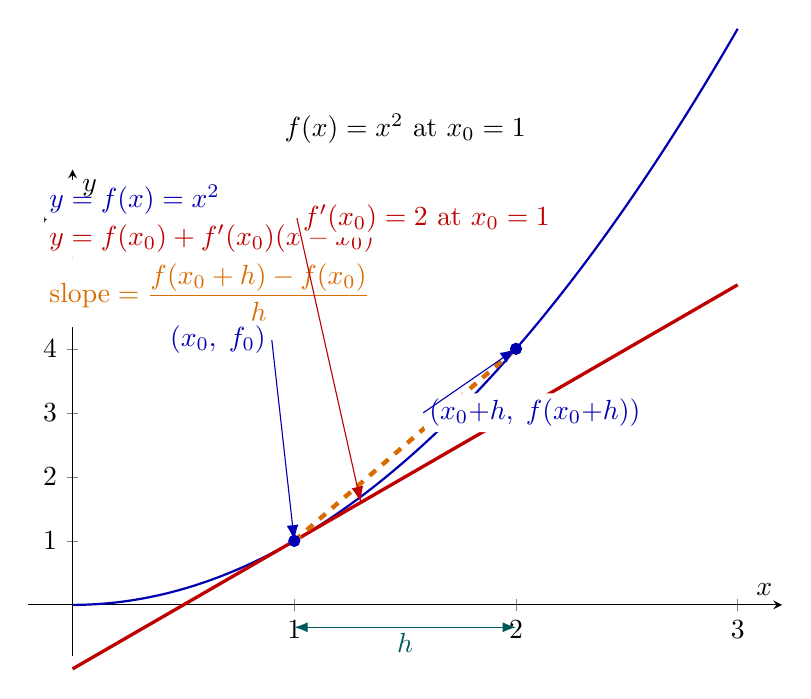
\begin{tikzpicture}
\begin{axis}[
    width=0.92\linewidth, height=0.64\linewidth,
    xmin=-0.2, xmax=3.2, ymin=-0.8, ymax=6.8,
    axis lines=middle,
    xlabel={$x$}, ylabel={$y$},
    xtick={0,1,2,3}, ytick={0,1,2,3,4,5,6},
    domain=0:3, samples=300,
    title={$f(x)=x^2$ at $x_0=1$},
    clip=false
]
% Parameters (precompute numerics only)
\pgfmathsetmacro{\xO}{1.0}
\pgfmathsetmacro{\hStep}{1.0}      % try 0.5 to see the secant approach the tangent
\pgfmathsetmacro{\xOne}{\xO+\hStep}
\pgfmathsetmacro{\fO}{\xO*\xO}
\pgfmathsetmacro{\fOne}{\xOne*\xOne}
\pgfmathsetmacro{\slope}{2*\xO}    % derivative at x0
\pgfmathsetmacro{\xMid}{(\xO+\xOne)/2}
% tangent sample point to aim arrow:
\pgfmathsetmacro{\xTan}{\xO+0.30}
\pgfmathsetmacro{\yTan}{\fO + \slope*(\xTan-\xO)}

% Function
\addplot[thick, color=blue!70!black] {x^2};

% Tangent line at x0
\addplot[very thick, color=red!75!black, domain=0:3] {\fO + \slope*(x-\xO)};

% Secant line
\addplot[dashed, ultra thick, color=orange!85!black] coordinates {(\xO,\fO) (\xOne,\fOne)};

% Points
\addplot[only marks, mark=*, mark options={fill=blue!70!black}, color=blue!70!black] coordinates {(\xO,\fO) (\xOne,\fOne)};

% Bracket for h
\addplot[<->,>=Latex, color=teal!70!black] coordinates {(\xO, -0.35) (\xOne, -0.35)};
\node[text=teal!70!black, fill=white, rounded corners=2pt, inner sep=1.4pt] at (axis cs:\xMid,-0.60) {$h$};

% --- Callouts (boxes away from curves) ---
% Equations (top-left, stacked, no arrows to reduce clutter)
\node[fill=white, rounded corners=2pt, inner sep=2pt, text=blue!70!black, anchor=north west] at (rel axis cs:0.02,0.98) {$y = f(x) = x^2$};
\node[fill=white, rounded corners=2pt, inner sep=2pt, text=red!75!black,  anchor=north west] at (rel axis cs:0.02,0.90) {$y = f(x_0) + f'(x_0)(x-x_0)$};
\node[fill=white, rounded corners=2pt, inner sep=2pt, text=orange!85!black, anchor=north west] at (rel axis cs:0.02,0.82) {$\displaystyle \text{slope} = \frac{f(x_0+h)-f(x_0)}{h}$};

% Point labels with arrows
\node (P0) [fill=white, rounded corners=2pt, inner sep=2pt, text=blue!70!black, anchor=west] at (rel axis cs:0.18,0.65) {$(x_0,\;f_0)$};
\draw[-{Latex[length=2mm]}, blue!70!black] (P0.east) -- (axis cs:\xO,\fO);

\node (P1) [fill=white, rounded corners=2pt, inner sep=2pt, text=blue!70!black, anchor=east] at (rel axis cs:0.82,0.50) {$(x_0{+}h,\;f(x_0{+}h))$};
\draw[-{Latex[length=2mm]}, blue!70!black] (P1.west) -- (axis cs:\xOne,\fOne);

% Tangent slope callout with arrow
\node (T0) [fill=white, rounded corners=2pt, inner sep=2pt, text=red!75!black, anchor=east] at (rel axis cs:0.70,0.90) {$f'(x_0)=2\text{ at }x_0=1$};
\draw[-{Latex[length=2mm]}, red!75!black] (T0.west) -- (axis cs:\xTan,\yTan);

\end{axis}
\end{tikzpicture}
\caption{For $f(x)=x^2$, the secant (orange) approaches the tangent (red) as $h\to 0$. Here $f'(1)=2$.}
\end{figure}

% ===================== Figure 2: f(x)=x^3 =====================
\begin{figure}[p]
\centering
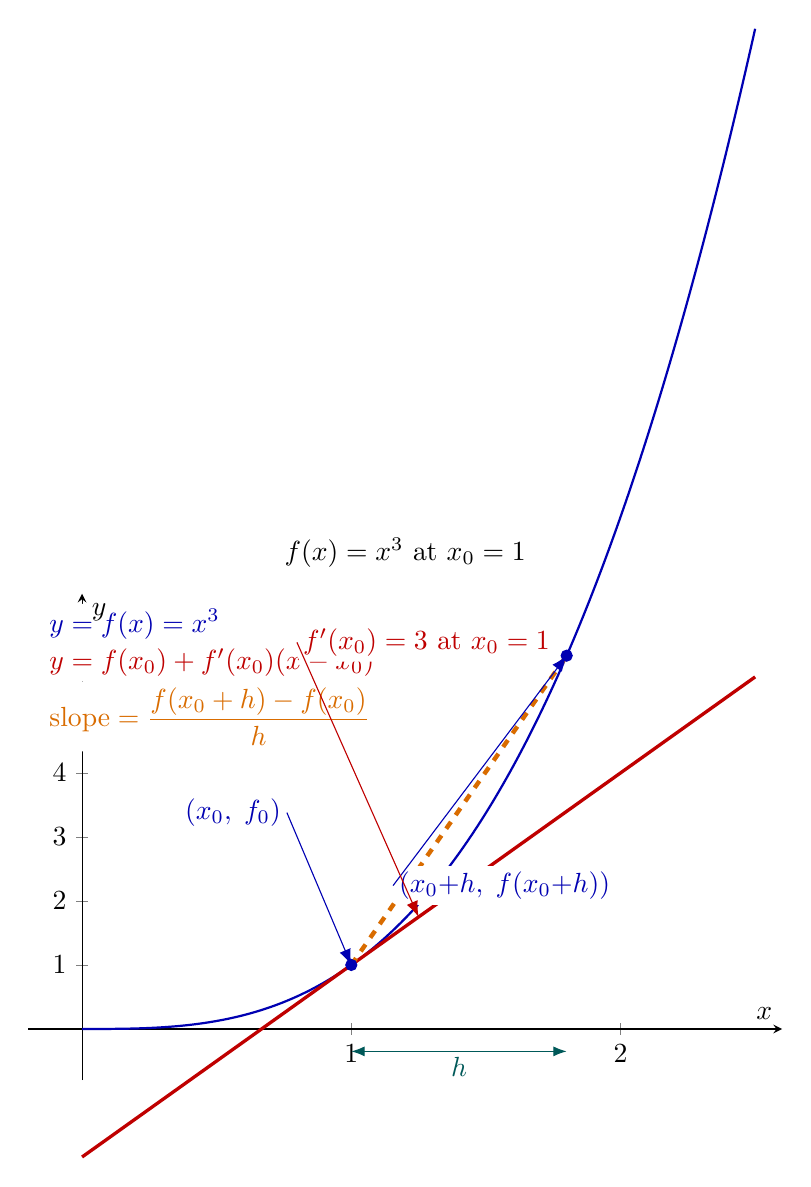
\begin{tikzpicture}
\begin{axis}[
    width=0.92\linewidth, height=0.64\linewidth,
    xmin=-0.2, xmax=2.6, ymin=-0.8, ymax=6.8,
    axis lines=middle,
    xlabel={$x$}, ylabel={$y$},
    xtick={0,1,2}, ytick={0,1,2,3,4,5,6},
    domain=0:2.5, samples=300,
    title={$f(x)=x^3$ at $x_0=1$},
    clip=false
]
% Parameters
\pgfmathsetmacro{\xO}{1.0}
\pgfmathsetmacro{\hStep}{0.8}
\pgfmathsetmacro{\xOne}{\xO+\hStep}
\pgfmathsetmacro{\fO}{\xO*\xO*\xO}
\pgfmathsetmacro{\fOne}{\xOne*\xOne*\xOne}
\pgfmathsetmacro{\slope}{3*\xO*\xO}   % derivative at x0
\pgfmathsetmacro{\xMid}{(\xO+\xOne)/2}
% tangent sample point for arrow:
\pgfmathsetmacro{\xTan}{\xO+0.25}
\pgfmathsetmacro{\yTan}{\fO + \slope*(\xTan-\xO)}

% Function
\addplot[thick, color=blue!70!black] {x^3};

% Tangent line
\addplot[very thick, color=red!75!black, domain=0:2.5] {\fO + \slope*(x-\xO)};

% Secant
\addplot[dashed, ultra thick, color=orange!85!black] coordinates {(\xO,\fO) (\xOne,\fOne)};

% Points
\addplot[only marks, mark=*, mark options={fill=blue!70!black}, color=blue!70!black] coordinates {(\xO,\fO) (\xOne,\fOne)};

% Bracket for h
\addplot[<->,>=Latex, color=teal!70!black] coordinates {(\xO, -0.35) (\xOne, -0.35)};
\node[text=teal!70!black, fill=white, rounded corners=2pt, inner sep=1.4pt] at (axis cs:\xMid,-0.60) {$h$};

% --- Callouts ---
\node[fill=white, rounded corners=2pt, inner sep=2pt, text=blue!70!black, anchor=north west] at (rel axis cs:0.02,0.98) {$y = f(x) = x^3$};
\node[fill=white, rounded corners=2pt, inner sep=2pt, text=red!75!black,  anchor=north west] at (rel axis cs:0.02,0.90) {$y = f(x_0) + f'(x_0)(x-x_0)$};
\node[fill=white, rounded corners=2pt, inner sep=2pt, text=orange!85!black, anchor=north west] at (rel axis cs:0.02,0.82) {$\displaystyle \text{slope} = \frac{f(x_0+h)-f(x_0)}{h}$};

\node (P0b) [fill=white, rounded corners=2pt, inner sep=2pt, text=blue!70!black, anchor=west] at (rel axis cs:0.20,0.55) {$(x_0,\;f_0)$};
\draw[-{Latex[length=2mm]}, blue!70!black] (P0b.east) -- (axis cs:\xO,\fO);

\node (P1b) [fill=white, rounded corners=2pt, inner sep=2pt, text=blue!70!black, anchor=east] at (rel axis cs:0.78,0.40) {$(x_0{+}h,\;f(x_0{+}h))$};
\draw[-{Latex[length=2mm]}, blue!70!black] (P1b.west) -- (axis cs:\xOne,\fOne);

\node (T0b) [fill=white, rounded corners=2pt, inner sep=2pt, text=red!75!black, anchor=east] at (rel axis cs:0.70,0.90) {$f'(x_0)=3\text{ at }x_0=1$};
\draw[-{Latex[length=2mm]}, red!75!black] (T0b.west) -- (axis cs:\xTan,\yTan);

\end{axis}
\end{tikzpicture}
\caption{For $f(x)=x^3$, the secant (orange) approaches the tangent (red) as $h\to 0$. Here $f'(1)=3$.}
\end{figure}

% ===================== Figure 3: f(x)=\sqrt{x} =====================
\begin{figure}[p]
\centering
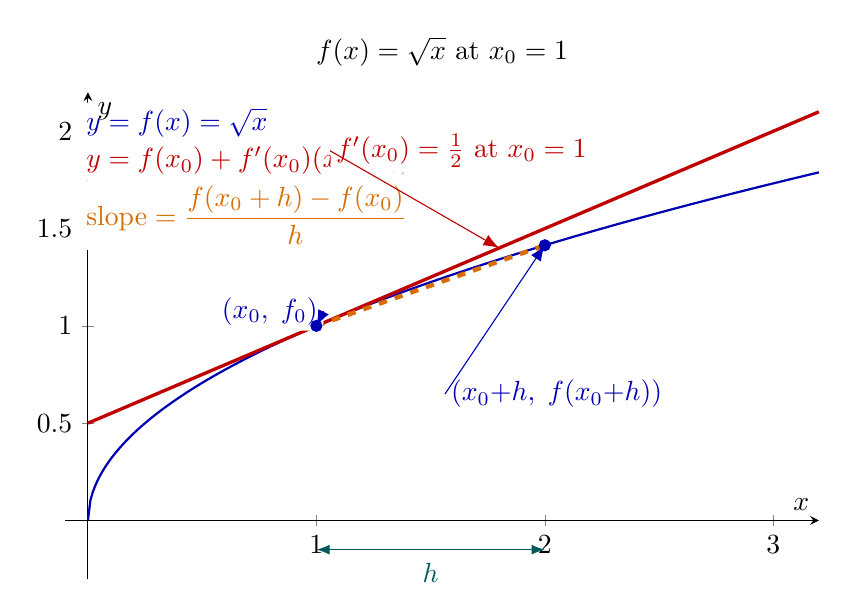
\begin{tikzpicture}
\begin{axis}[
    width=0.92\linewidth, height=0.64\linewidth,
    xmin=-0.1, xmax=3.2, ymin=-0.3, ymax=2.2,
    axis lines=middle,
    xlabel={$x$}, ylabel={$y$},
    xtick={0,1,2,3}, ytick={0,0.5,1,1.5,2},
    domain=0:3.2, samples=300,
    title={$f(x)=\sqrt{x}$ at $x_0=1$},
    clip=false
]
% Parameters
\pgfmathsetmacro{\xO}{1.0}
\pgfmathsetmacro{\hStep}{1.0}
\pgfmathsetmacro{\xOne}{\xO+\hStep}
\pgfmathsetmacro{\fO}{sqrt(\xO)}
\pgfmathsetmacro{\fOne}{sqrt(\xOne)}
\pgfmathsetmacro{\slope}{1.0/(2.0*sqrt(\xO))}  % derivative at x0
\pgfmathsetmacro{\xMid}{(\xO+\xOne)/2}
% tangent sample point:
\pgfmathsetmacro{\xTan}{\xO+0.80}
\pgfmathsetmacro{\yTan}{\fO + \slope*(\xTan-\xO)}

% Function
\addplot[thick, color=blue!70!black] {sqrt(x)};

% Tangent
\addplot[very thick, color=red!75!black, domain=0:3.2] {\fO + \slope*(x-\xO)};

% Secant
\addplot[dashed, ultra thick, color=orange!85!black] coordinates {(\xO,\fO) (\xOne,\fOne)};

% Points
\addplot[only marks, mark=*, mark options={fill=blue!70!black}, color=blue!70!black] coordinates {(\xO,\fO) (\xOne,\fOne)};

% Bracket for h
\addplot[<->,>=Latex, color=teal!70!black] coordinates {(\xO, -0.15) (\xOne, -0.15)};
\node[text=teal!70!black, fill=white, rounded corners=2pt, inner sep=1.4pt] at (axis cs:\xMid,-0.27) {$h$};

% --- Callouts ---
\node[fill=white, rounded corners=2pt, inner sep=2pt, text=blue!70!black, anchor=north west] at (rel axis cs:0.02,0.98) {$y = f(x) = \sqrt{x}$};
\node[fill=white, rounded corners=2pt, inner sep=2pt, text=red!75!black,  anchor=north west] at (rel axis cs:0.02,0.90) {$y = f(x_0) + f'(x_0)(x-x_0)$};
\node[fill=white, rounded corners=2pt, inner sep=2pt, text=orange!85!black, anchor=north west] at (rel axis cs:0.02,0.82) {$\displaystyle \text{slope} = \frac{f(x_0+h)-f(x_0)}{h}$};

\node (P0c) [fill=white, rounded corners=2pt, inner sep=2pt, text=blue!70!black, anchor=west] at (rel axis cs:0.20,0.55) {$(x_0,\;f_0)$};
\draw[-{Latex[length=2mm]}, blue!70!black] (P0c.east) -- (axis cs:\xO,\fO);

\node (P1c) [fill=white, rounded corners=2pt, inner sep=2pt, text=blue!70!black, anchor=east] at (rel axis cs:0.80,0.38) {$(x_0{+}h,\;f(x_0{+}h))$};
\draw[-{Latex[length=2mm]}, blue!70!black] (P1c.west) -- (axis cs:\xOne,\fOne);

\node (T0c) [fill=white, rounded corners=2pt, inner sep=2pt, text=red!75!black, anchor=east] at (rel axis cs:0.70,0.88) {$f'(x_0)=\tfrac12\text{ at }x_0=1$};
\draw[-{Latex[length=2mm]}, red!75!black] (T0c.west) -- (axis cs:\xTan,\yTan);

\end{axis}
\end{tikzpicture}
\caption{For $f(x)=\sqrt{x}$, the secant (orange) approaches the tangent (red) as $h\to 0$. Here $f'(1)=\tfrac12$.}
\end{figure}

\end{document}
